
    \subsection*{Single Layer: Visualizing our Components}
    
        Now, rather than analyzing a single neuron, we will analyze a single \textbf{layer}.
        
        \begin{figure}[H]
            \centering
            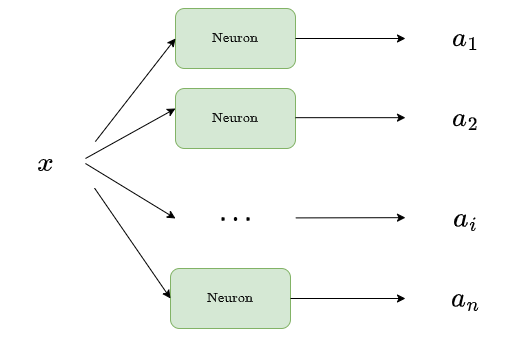
\includegraphics[width=80mm,scale=0.4]{images/nn_images/general_layer.png}
            \caption*{Our first layer.}
        \end{figure}
        
        In order to \textbf{analyze} this layer, we have to open back up the \textbf{abstraction}:
        
        \begin{figure}[H]
            \centering
            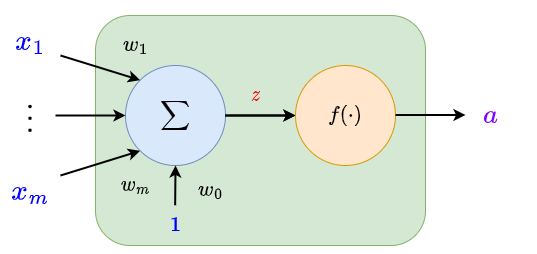
\includegraphics[width=80mm,scale=0.4]{images/nn_images/neuron_inside.png}
            \caption*{Each of those neurons looks like this.}
        \end{figure}
        
        There are two important pieces of \textbf{information} we're hiding:
        
        \begin{itemize}
            \item We have two components inside of our neuron.
            
            \item We have many inputs $x_i$ for one neuron.
        \end{itemize}
        
        The first piece of information is easier to visualize: we just replace each neuron with the two components.
        
        \begin{figure}[H]
            \centering
            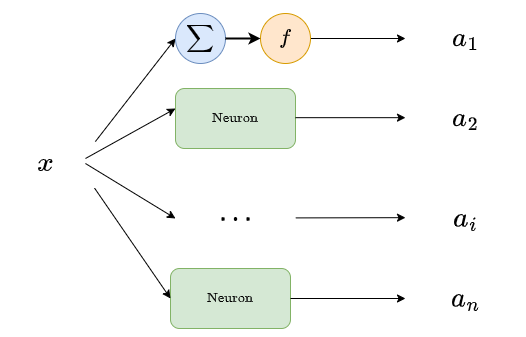
\includegraphics[width=80mm,scale=0.4]{images/nn_images/replace_one_neuron.png}
            \caption*{Replacing one neuron...}
        \end{figure}
        
        \begin{figure}[H]
            \centering
            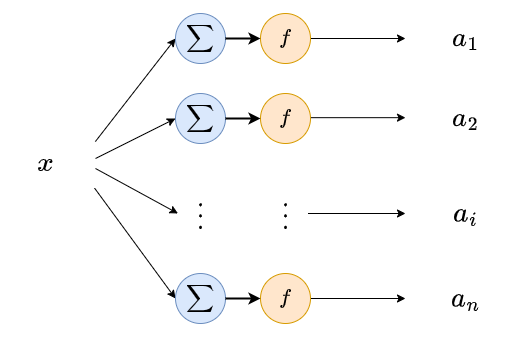
\includegraphics[width=80mm,scale=0.4]{images/nn_images/replace_all_neurons.png}
            \caption*{Replacing all neurons!}
        \end{figure}
    
    \subsection*{Single Layer: Visualizing our Inputs}
    
        The second piece of information is much more difficult: we show all of the $x_i$ outputs.
        
        \begin{figure}[H]
            \centering
            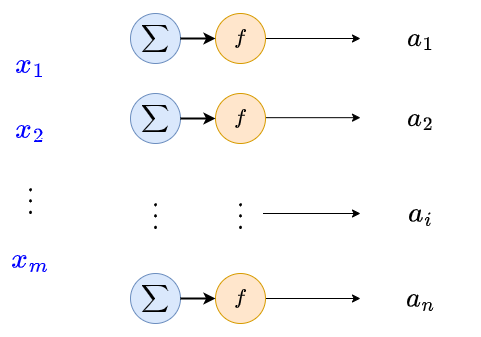
\includegraphics[width=80mm,scale=0.4]{images/nn_images/layers_with_input.png}
        \end{figure}
        
        Now we have to draw the arrow for each input.
        
        \begin{figure}[H]
            \centering
            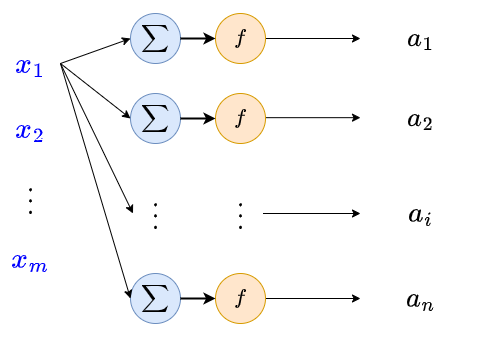
\includegraphics[width=80mm,scale=0.4]{images/nn_images/layers_one_neuron_input.png}
            \caption*{Every neuron receives the first input.}
        \end{figure}
        
        \begin{figure}[H]
            \centering
            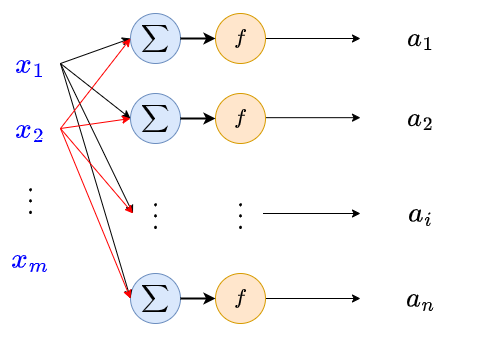
\includegraphics[width=80mm,scale=0.4]{images/nn_images/layers_two_neuron_input.png}
            \caption*{Every neuron receives the second input, too. This is getting messy...}
        \end{figure}
        
        \begin{figure}[H]
            \centering
            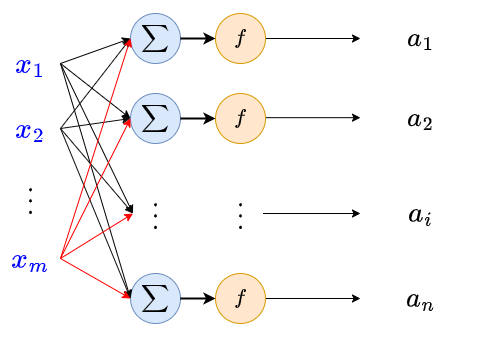
\includegraphics[width=80mm,scale=0.4]{images/nn_images/layers_all_neuron_input.png}
            \caption*{The completed version: this is hard to look at.}
        \end{figure}
        
        Don't worry if this looks \textbf{confusing}! It's natural for it to be \textbf{hard} to read: the only thing you need to know is that we pair \textbf{every} input with \textbf{every} neuron.
        
        This is our \textbf{final} view of this layer: because each of our $m$ inputs has to go to every of $n$ neurons, we end up with $mn$ different \textbf{weights}.
        
        This is a ton of \textbf{information}, and its only one layer! This shows how \textbf{complex} a neural network can be, just by \textbf{combining} simple neurons.
        
        Note that this is a \textbf{fully connected} network: not all networks are FC.\\
        
        \begin{definition}
            A layer is \vocab{fully connected} if every neuron has the \purp{same input vector}.
        \end{definition}
        
        \miniex If one of our neurons \textbf{ignored} $x_1$, but the others did \textbf{not}, the layer would not be \textbf{fully connected}.
        
    \subsection*{Dimensions of a layer}
    
        Now that we've seen the \textbf{full} view, we can \textbf{analyze} it. Our goal is to create a more \textbf{useful} and \textbf{accurate} simplification.
        
        Our first point: note that the input and output have a \textbf{different} dimensions!\\
        
        \begin{clarification}
            A \vocab{layer} can have a different \gren{input} and \purp{output} dimension. In fact, they are completely \purp{separate} variables.
        \end{clarification}
        
        This is because \textbf{every} input variable is allowed to be applied to the \textbf{same} neuron: 
            
        \miniex You can have one neuron of the form
        
        \begin{equation*}
            z = 
            \begin{bmatrix}
                w_1 & w_2 & w_3
            \end{bmatrix}
            \begin{bmatrix}
                x_1\\x_2\\x_3
            \end{bmatrix}
            +
            w_0
        \end{equation*}
        
        In this case, our neuron has \textbf{one} output variable $f(z)$, but \textbf{three} inputs $x_1,x_2,x_3$.
        
        Thus, our output dimension has been separated from our input dimension. Instead, it is the number of neurons.
        
        So, in general, we can say:\\
        
        \begin{notation}
            A \vocab{layer} has two associated \purp{dimensions}: the \gren{input} dimension \vocab{$m$} and the \gren{output} dimension \vocab{$n$}.
            
            \begin{itemize}
                \item The \gren{input} dimension \vocab{$m$} is based on the vector output from the \purp{previous layer}: $x \in \RR^m$
                
                \item The \gren{output} dimension \vocab{$n$} is equal to the \purp{number of neurons} in the \gren{current} layer: $A \in \RR^n$
            \end{itemize}
        \end{notation}
        
        \miniex Suppose you have an \textbf{input} vector $x=[x_1, x_2, x_3]$ and two \textbf{neurons}. The dimensions are $m=3$, and $n=2$.
    
        \begin{figure}[H]
            \centering
            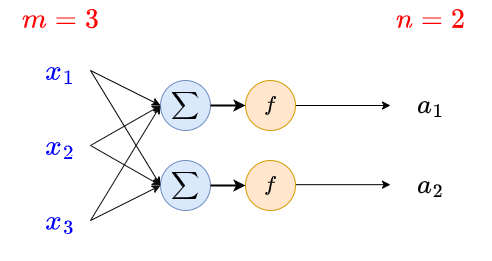
\includegraphics[width=80mm,scale=0.4]{images/nn_images/dimensions_network.png}
            \caption*{The input dimension and output dimensions are \textbf{separate}.}
        \end{figure}
        
    \subsection*{The known objects of our layer}
    
        So, we know we have two objects so far:
        
        \begin{itemize}
            \item Our \textbf{input} vector $x \in \RR^m$
            
            \item Our \textbf{output} vector $A \in \RR_n$

        \end{itemize}
        
        Where they each take the form
        
        \begin{equation}
            x = 
                \begin{bmatrix}
                  x_1\\x_2\\ \vdots \\ x_m
                \end{bmatrix}
            \qquad \qquad \qquad
            A =
            \begin{bmatrix}
                a_1\\a_2\\ \vdots \\ a_n
            \end{bmatrix}
        \end{equation}
        
        But, there are a couple other things we haven't \textbf{generalized} for our entire \textbf{layer}:
        
        \begin{itemize}
            \item Our weights 
            \item Our offsets
            \item Our preactivation
        \end{itemize}
        
    \subsection*{The other variables of our layer: weights and offsets}
        
        First, our \textbf{weights}: each neuron has its own vector of weights $w \in \RR^m$.
            \note{The dimension needs to match $x$ so we can compute $w^Tx$.}
            
        \begin{equation}
            w = 
            \begin{bmatrix}
              w_1\\w_2\\ \vdots \\ w_m
            \end{bmatrix}
        \end{equation}
        
        To distinguish them from each other, we'll represent the $\nth{i}$ neuron's weights as $\vec{w}_i$.
        
        \begin{equation}
            \vec{w}_i = 
            \begin{bmatrix}
              w_{1i}\\w_{2i}\\ \vdots \\ w_{mi}
            \end{bmatrix}
        \end{equation}
            
        Each needs to be used to \textbf{compute} $a_i$, but having so many objects is annoying.
        
        Remember that, when we had \textbf{multiple} data points $\exi$, we worked with them at the \textbf{same time} by stacking them in a \textbf{matrix}. Let's do the same here:
        
        \begin{equation}
            W = 
            \overbrace{
                \begin{bmatrix}
                  \vec{w}_1 & \vec{w}_2 & \cdots & \vec{w}_n
                \end{bmatrix}
            }^{\text{Each neuron has a weight vector}}
        \end{equation}
        
        If we expand it out, we get a full matrix...
        
        \begin{equation}
            W = 
            \overbrace{
                \begin{bmatrix}
                  w_{\red{11}} & w_{\red{12}} & \cdots & w_{\red{1n}} \\
                  w_{\red{21}} & w_{\red{22}} & \cdots & w_{\red{2n}} \\
                  \vdots       & \vdots       & \ddots & \vdots \\
                  w_{\red{m1}} & w_{\red{m1}} & \cdots & w_{\red{mn}} \\
                \end{bmatrix}
            }^{\red{n} \text{ neurons}}
            \bigggrB{70pt} \red{m} \text{ inputs}
        \end{equation}
        
        This is our \textbf{weight matrix} $W$: it's an $(m \times n)$ matrix. It contains all of our $mn$ weights, sorted by
        
        \begin{itemize}
            \item \vocab{Input variable} (row)
            \item \vocab{Neuron} (column)
        \end{itemize} 
        
        We can do this for our \textbf{offsets} too: thankfully, there is only \textbf{one} offset per neuron, so we can write:
        
        \begin{equation}
            W_0 = 
                \begin{bmatrix}
                  w_{\red{01}} \\ w_{\red{02}} \\ \vdots \\ w_{\red{0n}}
                \end{bmatrix}
            \bigggrB{70pt} \text{Each neuron has an offset}
        \end{equation}
        
        This is our offset vector, with the shape $(n \times 1)$.\\
        
        \begin{notation}
            We can store our \vocab{weights} and \vocab{offsets} as \purp{matrices}:
            
            \begin{itemize}
                \item \purp{Weight} matrix $W$ has the shape $\blu{(m \times n)}$
                
                \item \purp{Offset} matrix $W_0$ has the shape $\blu{(n \times 1)}$
            \end{itemize}
        \end{notation}
        
        These matrices give us a tidy way to understand all of this mess:
        
        \begin{figure}[H]
            \centering
            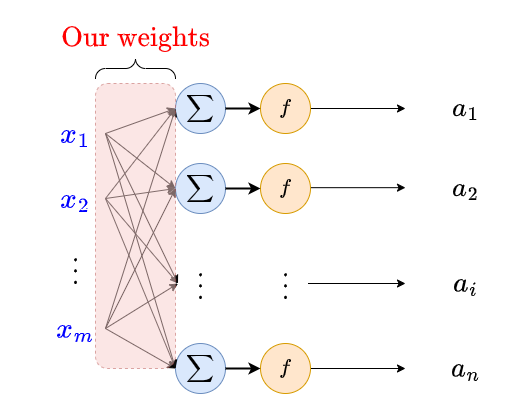
\includegraphics[width=80mm,scale=0.4]{images/nn_images/weights_highlighted.png}
        \end{figure}
        
        Now that we understand it, we'll \textbf{hide} those weights again, for readability.
        
        \begin{figure}[H]
            \centering
            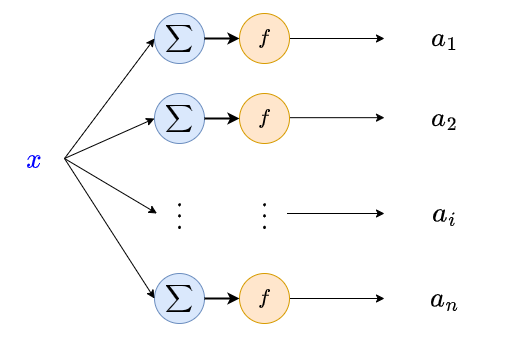
\includegraphics[width=80mm,scale=0.4]{images/nn_images/remove_input.png}
        \end{figure}
        
    
    \subsection*{Pre-activation}
    
        Now, all that remains is the pre-activation $z$.
        
        Before, we did 
        
        \begin{equation}
            w^Tx + w_0 = z
        \end{equation}
        
        Because we so carefully kept our weights and offsets separate, we can still do this!
        
        \begin{equation}
            W^Tx + W_0 = Z
        \end{equation}
        
        This pre-activation vector $Z$ contains all of the outputs of our linear components:
        
        \begin{equation}
            Z = 
            \begin{bmatrix}
              z_1 \\ z_2 \\ \vdots \\ z_n
            \end{bmatrix}
        \end{equation}
        
        On our diagram, we can see it here:
        
        \begin{figure}[H]
            \centering
            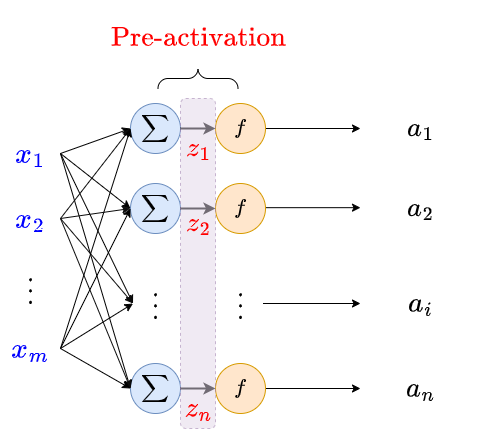
\includegraphics[width=80mm,scale=0.4]{images/nn_images/pre_activation.png}
            \caption*{This section is what $Z$ details with.}
        \end{figure}
        
        And we can connect this to our activation: each $a_i$ is the result of running our function $f$ on $z_i$:
            \note{Because we run the function on each element in $Z$, we call this an \textbf{element-wise} use of our function.}
        
        \begin{equation}
            A = 
            \red{f}(Z)=
            \begin{bmatrix}
              \red{f}(z_1) \\ \red{f}(z_2) \\ \vdots \\ \red{f}(z_n)
            \end{bmatrix}
        \end{equation}
        
    \subsection*{Summary of layer}
    
        So, we can now break our our layer up into pieces:\\
        
        \begin{notation}
            Our \vocab{layer} is a \purp{function} that takes in $x \in \RR^m$, and returns $A \in \RR^n$.
            
            It is defined by:
            
            \begin{itemize}
                \item \vocab{Dimensions}: $m$ for \gren{input}, $n$ for \gren{output} (number of neurons)
            \end{itemize}
            
            And our different \purp{matrices}:
            
            \begin{itemize}
                \item \vocab{Input}: a \purp{column vector} $X$ in the shape $(\blu{m} \times 1)$
            
                \item \vocab{Weights}: a \purp{matrix} $W$ in the shape $(\blu{m} \times \red{n})$
                
                \item \vocab{Offset}: a \purp{column vector} $W_0$ in the shape $(\red{n} \times 1)$
                
                \item \vocab{Pre-activation}: a \purp{column vector} $Z$ in the shape $(\red{n} \times 1)$
                
                \item \vocab{Activation}: a \purp{column vector} $A$ in the shape $(\red{n} \times 1)$
            \end{itemize}
        \end{notation}
        
        We've now accomplished our goal: \textbf{simplify} the layer into its \textbf{base} components, without losing any crucial \textbf{information}.
        
        We've can represent an entire layer like this:
        
        \begin{figure}[H]
            \centering
            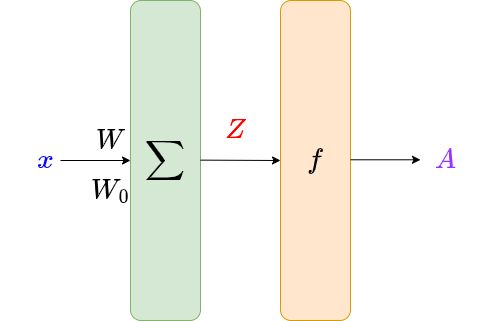
\includegraphics[width=100mm,scale=0.4]{images/nn_images/layer_simplified.png}
        \end{figure}
        
        Note how similar this looks to a \textbf{single} neuron: this works because the neurons in a \textbf{layer} are in \textbf{parallel}!
        
        \begin{figure}[H]
            \centering
            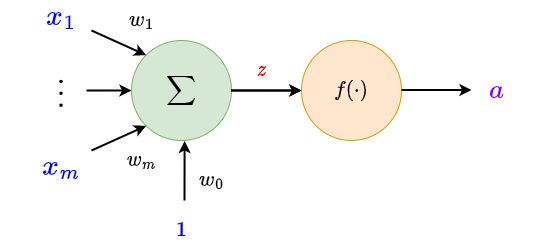
\includegraphics[width=100mm,scale=0.4]{images/nn_images/full_neuron.png}
        \end{figure}
        
        The math is very similar as well:\\
        
        \begin{definition}
            Our \vocab{layer} can be represented by
            
            \begin{itemize}
                \item A \vocab{linear} component that takes in $x$, and outputs \purp{pre-activation} $Z$:
                
                \begin{equation*}
                    Z = W^T x + W_0
                \end{equation*}
                
                \item A (potentially nonlinear) \vocab{activation} component that takes in $Z$, and outputs \purp{activation} $A$:
                
                \begin{equation*}
                    A = f(Z)
                \end{equation*}
                
            \end{itemize}
        
            When we \purp{compose} them together, we get
                
                \begin{equation*}
                    A = f(Z) = f \Big( W^Tx+W_0 \Big)
                \end{equation*}
        \end{definition}
        